% =====================================================================
%  paper.tex -- AI for Mathematics : Reliability through Semantic Reduction
%  Challenge C2 (AI4Math) -- submittable LaTeX academic paper
%  Compile:  pdflatex paper  &&  bibtex paper  &&  pdflatex paper  &&  pdflatex paper
% =====================================================================
\documentclass[11pt,a4paper]{article}

% ------------------------- packages --------------------------------
\usepackage[margin=1in]{geometry}
\usepackage{amsmath,amssymb,amsthm}
\usepackage{graphicx}
\usepackage{xcolor}
\usepackage{booktabs}
\usepackage{caption}
\usepackage{subcaption}
\usepackage{enumitem}
\usepackage{microtype}
\usepackage[hidelinks]{hyperref}
\usepackage[numbers,sort&compress]{natbib}
\usepackage{tikz}
\usetikzlibrary{positioning,arrows.meta,shapes.geometric,calc}

% ------------------------- theorem environments --------------------
\theoremstyle{definition}
\newtheorem{definition}{Definition}[section]
\newtheorem{remark}{Remark}[section]
\theoremstyle{plain}
\newtheorem{theorem}{Theorem}[section]
\newtheorem{proposition}{Proposition}[section]

% ------------------------- metadata --------------------------------
\title{\bfseries From Natural Language to Verifiable Reasoning:\\
A Semantic Reduction Framework for Reliable AI Mathematics}
\author{
  Ruan Yihan\\
  \small School of Software Engineering, Zhengzhou Sias University, China\\
  \small \texttt{ruan.yihan@example.com}
}
\date{\today}

\begin{document}

\maketitle

% =====================================================================
%  ABSTRACT
% =====================================================================
\begin{abstract}
\noindent
Large language models (LLMs) exhibit impressive fluency in mathematical reasoning, yet their
natural-language derivations are notoriously difficult to verify: a model may produce a step that
\emph{looks} correct while being subtly wrong. Existing reliability responses---search-plus-verification,
formal proof, and reproducible evaluation---typically treat verification as a final, post-hoc gate.
In this paper we argue that reliability cannot rest on final verification alone; a \emph{semantic
reduction layer} must be introduced between informal natural-language reasoning and formal verification.
We make three contributions. First, we formalize a three-layer decomposition of AI mathematical
reasoning---generation, semantic reduction, and verification---and identify the middle layer as the
principal locus of failure. Second, we propose a concrete framework built on a typed intermediate
representation (IR), a four-stage \emph{natural-language $\rightarrow$ IR $\rightarrow$ verification
$\rightarrow$ rendering} pipeline, and a bidirectional-consistency contract that preserves
interpretability and traceability. Third, we contribute two auditable artifacts: a taxonomy of four
semantic-reduction failure modes (ambiguity, missing typing, non-invertibility, and semantic drift) and
a graded \emph{Verifiability Certificate} (levels V0--V4) that lets researchers compare any AI4Math
system on a common reliability scale. We anchor the framework in three recent case studies
(AlphaProof, an LLM research agent, and counterexample construction) and design an evaluation protocol
for GSM8K/MATH with accuracy, verifiability, and consistency metrics. We close by stating the
boundaries of the framework and its extension to general reasoning and agentic systems.
\end{abstract}

% keywords
\noindent\textbf{Keywords:} AI for mathematics; reliability; semantic reduction; formal verification;
intermediate representation; verifiability certificate

% =====================================================================
%  1. INTRODUCTION
% =====================================================================
\section{Introduction}
\label{sec:intro}

Mathematics has long been regarded as the pinnacle of purely human intelligence, relying on insight,
intuition, and rigorous logic to prove conjectures and create theories
\cite{chen2025reshaping}. With the recent breakthroughs of deep learning and large language models
built on the Transformer architecture \cite{vaswani2017}, a
natural question has emerged: how will the combination of AI and mathematics reshape the way we explore
the mathematical world? The literature records remarkable successes across the full spectrum of
mathematical activity---discovering hidden relations between knot invariants \cite{davies2021},
discovering faster matrix-multiplication algorithms \cite{fawzi2022}, constructing counterexamples in
combinatorics \cite{wagner2021}, and attaining medal-level performance in formal olympiad
mathematics \cite{trinh2024,hubert2026,chervonyi2025}.

At the same time, a persistent and fundamental concern shadows these achievements: \emph{trust}.
Modern LLMs are probabilistic, untyped, and trained to be fluent rather than to be sound; they routinely
emit derivations that are locally plausible but globally invalid, a failure commonly described as
``hallucination.'' In mathematics, where a single unjustified step invalidates a whole proof, such
failures are not cosmetic---they are fatal. The core reliability problem of AI for mathematics
(AI4Math) can therefore be stated crisply: \emph{natural-language reasoning is not directly
verifiable.}

The research community has responded with what we call the \emph{reliability triad}:
(i)~\emph{search + verification}, in which a generator proposes and a verifier checks;
(ii)~\emph{formalization}, in which reasoning is carried out inside a proof assistant such as Lean or
Coq whose kernel performs machine-checkable verification \cite{moura2021,polu2020,hubert2026}; and
(iii)~\emph{reproducible evaluation}, in which claims are backed by released code, data, and metrics
\cite{cobbe2021,hendrycks2021}. Each of these responses, however, tends to treat verification as a
\emph{final gate} applied after generation. In this paper we argue that this is insufficient.

Our central thesis is that \textbf{reliability cannot rely solely on final verification; it requires a
dedicated \emph{semantic reduction} layer that converts informal reasoning into a machine-checkable
form}. When such a layer is absent or unstable, the verifier has \emph{no handle to grasp}---there is no
computable object to check, and hallucinations persist undetected. We therefore place semantic reduction
at the center of the reliability problem, rather than treating it as an implementation detail.

Concretely, we make the following contributions.
\begin{enumerate}[leftmargin=*]
  \item \textbf{A three-layer decomposition.} We formalize AI mathematical reasoning as a pipeline of
  \emph{generation}, \emph{semantic reduction}, and \emph{verification}, and argue---with evidence from
  recent systems---that the semantic reduction layer is the principal source of system failure.
  \item \textbf{A semantic-reduction framework.} We propose a concrete architecture built on a typed
  intermediate representation (IR), a four-stage pipeline
  (natural language $\rightarrow$ IR $\rightarrow$ verification $\rightarrow$ rendering), and a
  bidirectional-consistency contract ensuring interpretability and traceability.
  \item \textbf{An auditable reliability taxonomy.} We introduce a taxonomy of four semantic-reduction
  failure modes and a graded \emph{Verifiability Certificate} (V0--V4), giving the community a common
  scale on which any AI4Math system can be audited and compared.
  \item \textbf{Anchoring case studies and an evaluation protocol.} We map three representative systems
  onto the framework and design a concrete evaluation protocol over GSM8K and MATH with
  accuracy, verifiability, and consistency metrics.
\end{enumerate}

The remainder of the paper is organized as follows. Section~\ref{sec:model} presents the problem and the
three-layer model. Section~\ref{sec:related} reviews related work. Section~\ref{sec:framework} develops
the proposed framework, including the failure taxonomy and the Verifiability Certificate.
Section~\ref{sec:analysis} analyzes three case studies through the lens of the framework, and
Section~\ref{sec:experiments} designs the evaluation protocol. Section~\ref{sec:applications} discusses
applications, Section~\ref{sec:discussion} states limitations and boundaries, and Section~\ref{sec:concl}
concludes.

% =====================================================================
%  2. PROBLEM AND THREE-LAYER MODEL
% =====================================================================
\section{Problem Formulation and the Three-Layer Model}
\label{sec:model}

\subsection{The reliability problem}
\label{sec:problem}

Let $\mathcal{Q}$ be a mathematical question and let $\mathcal{M}$ be an LLM-based reasoning system.
We write the system output as $\hat{p} = \mathcal{M}(q)$, a natural-language ``proof'' or solution
attempt. We wish to certify a claim of the form
\begin{equation}
  \label{eq:reliability}
  \mathsf{Certify}\big(\hat{p}\ \text{is a correct solution of}\ q\big),
\end{equation}
where \emph{correctness} means that every inference step is valid and the final conclusion follows from
the stated assumptions.

The difficulty is that $\hat{p}$ is \emph{informal}: it is composed of natural-language tokens, is
untyped, and its semantics are not grounded in any computational object. As a consequence, a verifier
cannot, in general, mechanically decide whether \eqref{eq:reliability} holds. This is the fundamental
obstacle that motivates an intermediate representation.

\subsection{Three-layer decomposition}
\label{sec:threelayer}

We decompose any AI4Math system into three layers, following and sharpening the outline proposed in the
course material \cite{chen2025reshaping}.

\begin{definition}[Generation Layer]
The \emph{generation layer} $\mathcal{G}$ takes a question $q$ and produces a natural-language chain of
reasoning $\hat{p} = \mathcal{G}(q)$, e.g.\ a chain-of-thought sequence \cite{wei2022}. Its outputs are
probabilistic, untyped, and informal.
\end{definition}

\begin{definition}[Semantic Reduction Layer]
The \emph{semantic reduction layer} $\mathcal{R}$ maps the informal output $\hat{p}$ to a structured,
machine-readable representation $r = \mathcal{R}(\hat{p})$ drawn from a target class
$\mathcal{T}$. Typical targets include: (i)~logical expressions (first-order or higher-order logic);
(ii)~executable programs (Python or a domain-specific language); (iii)~proof objects accepted by a proof
assistant; and (iv)~typed intermediate representations (typed IR). The theoretical grounding for the
identity between \emph{propositions} and \emph{types} is the Curry--Howard correspondence
\cite{howard1980}.
\end{definition}

\begin{definition}[Verification Layer]
The \emph{verification layer} $\mathcal{V}$ operates on the structured representation $r$ and checks
properties such as consistency, derivability, factual grounding, and constraint satisfaction, using
mechanized tools (proof assistants, SMT solvers, symbolic checkers). Its verdict is
$\mathcal{V}(r) \in \{\mathsf{accept},\mathsf{reject}\}$.
\end{definition}

The overall system is the composition
\begin{equation}
  \label{eq:pipeline}
  q \;\xrightarrow{\;\mathcal{G}\;}\; \hat{p} \;\xrightarrow{\;\mathcal{R}\;}\; r
  \;\xrightarrow{\;\mathcal{V}\;}\; \{\mathsf{accept},\mathsf{reject}\}.
\end{equation}

\subsection{The bottleneck: semantic reduction}
\label{sec:bottleneck}

Our key observation---drawn from a comparative reading of recent systems
\cite{hubert2026,trinh2024,romera2024,wagner2021}---is that \emph{current systems fail predominantly in
the semantic reduction layer, not in the generation or verification layers}.

\begin{remark}
Verification depends on a \emph{computable object}. When the natural-language-to-formal-object
reduction is unstable, the verifier is left with ``no handle to verify'': there is no well-typed
representation to check, so \eqref{eq:reliability} cannot even be posed, and hallucinations escape
detection.
\end{remark}

This observation has a methodological consequence: improving the verifier alone cannot close the
reliability gap if the reduction feeding it is unreliable. The framework we propose in
Section~\ref{sec:framework} therefore invests its design effort in the semantic reduction layer.

% =====================================================================
%  3. RELATED WORK
% =====================================================================
\section{Related Work}
\label{sec:related}

\subsection{Chain-of-thought and program-of-thought}
\label{sec:rel-cot}

Chain-of-thought (CoT) prompting elicits explicit reasoning traces from LLMs and markedly improves
performance on arithmetic and symbolic tasks \cite{wei2022}. Program-of-thought moves one step toward
verifiability by instructing the model to emit executable code rather than prose, so that the reasoning
can be executed by an interpreter. Both, however, leave the \emph{translation} between informal language
and the executable form implicit and ungoverned.

\subsection{Tool-augmented and neuro-symbolic systems}
\label{sec:rel-tools}

Tool-augmented LLMs (code interpreters, calculators, symbolic engines) combine the pattern-recognition
of neural models with the exactness of symbolic tools. Open language models specialized for mathematics,
such as LEMMA \cite{azerbayev2024}, additionally provide reproducible baselines for studying how
pretraining data shape mathematical competence. The DeepMind line of systems---AlphaTensor
\cite{fawzi2022}, FunSearch \cite{romera2024}, AlphaGeometry \cite{trinh2024}---exemplifies the
neuro-symbolic paradigm, in which a neural model proposes and a symbolic component validates or scores.
These systems are highly successful on their targeted problem classes but are engineered per task; our
framework abstracts their common skeleton into a reusable semantic-reduction layer.

\subsection{Proof assistants and formal verification}
\label{sec:rel-formal}

Interactive theorem provers (ITP) such as Coq, Isabelle, and Lean provide a trusted kernel that
machine-checks each proof step \cite{moura2021,polu2020}. The formalization of major results (e.g.\ the
four-color theorem \cite{appel1977} in the wider context of machine proof) and the construction of
large formal libraries (Lean's \texttt{mathlib}) create the infrastructure on which reliable AI theorem
proving can be built. AlphaProof \cite{hubert2026} and AlphaGeometry2 \cite{chervonyi2025} demonstrate
that neural search coupled with a Lean kernel can reach olympiad-medal performance while guaranteeing
logical soundness. Our framework treats these formal systems as the \emph{verification layer} and
emphasizes the often-neglected reduction that feeds them.

\subsection{Reliability and reproducibility of AI mathematical claims}
\label{sec:rel-repro}

Benchmarks such as GSM8K \cite{cobbe2021} and MATH \cite{hendrycks2021} measure answer accuracy but not
proof soundness; recent work on mathematical creativity and on evaluating LLM capabilities
\cite{chen2025deepmath,frieder2023} highlights that fluency is decoupled from validity. Reproducible
evaluation---releasing code, data, and configuration \cite{silver2018,sutton2018}---is a necessary but
not sufficient condition for reliability. The graded certificate we propose
(Section~\ref{sec:certificate}) makes this distinction explicit.

% =====================================================================
%  4. PROPOSED FRAMEWORK
% =====================================================================
\section{A Semantic-Reduction Framework for Reliable AI Mathematics}
\label{sec:framework}

\subsection{Structured intermediate representation (IR)}
\label{sec:ir}

The cornerstone of the framework is a \emph{typed intermediate representation}. A well-designed IR must
satisfy four requirements:
\begin{enumerate}[leftmargin=*]
  \item \textbf{Type system:} every term carries a type, so ill-formed constructions are rejected by
  construction.
  \item \textbf{Operational semantics:} the meaning of each term is defined by explicit execution rules,
  giving the verifier a computational handle.
  \item \textbf{Constraint system:} the IR can express invariants, side conditions, and target
  properties to be checked.
  \item \textbf{Compositionality:} terms compose into graphs or trees (ASTs, workflow graphs), enabling
  modular verification and reuse.
\end{enumerate}
Concrete instantiations of the IR include domain-specific languages (DSLs), abstract syntax trees
(ASTs), proof objects, and workflow graphs. Choosing an IR is a design decision that trades expressiveness
against checkability.

\subsection{The four-stage pipeline}
\label{sec:pipeline}

We propose the standard pipeline:
\begin{equation}
\label{eq:pipelinestages}
\text{Natural Language} \;\xrightarrow{\;\text{reduce}\;}\;
\text{Typed IR} \;\xrightarrow{\;\text{verify}\;}\;
\text{Verification} \;\xrightarrow{\;\text{render}\;}\;
\text{Natural Language Rendering}.
\end{equation}
Two ideas are central. First, \emph{natural language is only an interface}: the human-visible prose is a
rendering of the IR, not the reasoning itself. Second, \emph{the IR is the execution core}: all
reliability-relevant computation happens on the typed structure. Figure~\ref{fig:pipeline} illustrates
the pipeline together with the two consistency directions.

\begin{figure}[t]
\centering
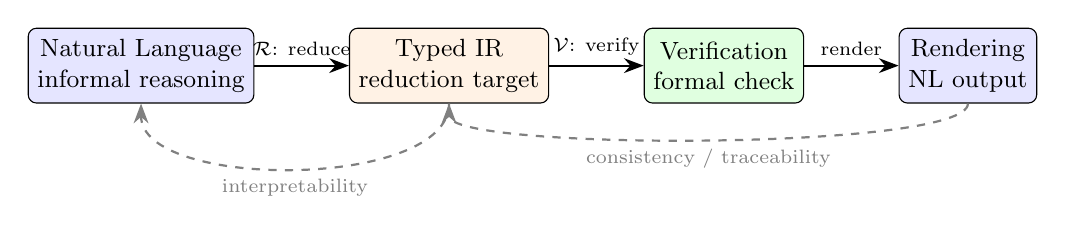
\begin{tikzpicture}[
  node distance=1.1cm and 1.2cm,
  box/.style={draw, rounded corners=3pt, minimum height=0.95cm, align=center, font=\small, fill=#1},
  box/.default=blue!8,
  arr/.style={-{Stealth[length=2.5mm]}, thick}
]
  \node[box=blue!10] (nl) {Natural Language\\\small informal reasoning};
  \node[box=orange!10, right=of nl] (ir) {Typed IR\\\small reduction target};
  \node[box=green!12, right=of ir] (ver) {Verification\\\small formal check};
  \node[box=blue!10, right=of ver] (ren) {Rendering\\\small NL output};
  \draw[arr] (nl) -- node[above,font=\scriptsize]{$\mathcal{R}$: reduce} (ir);
  \draw[arr] (ir) -- node[above,font=\scriptsize]{$\mathcal{V}$: verify} (ver);
  \draw[arr] (ver) -- node[above,font=\scriptsize]{render} (ren);
  \draw[arr, gray, dashed] (ren.south) .. controls ($(ren.south)+(0,-0.6)$) and ($(ir.south)+(0,-0.6)$) ..
        node[below, font=\scriptsize, text=gray]{consistency / traceability} (ir.south);
  \draw[arr, gray, dashed] (ir.south) .. controls ($(ir.south)+(0,-1.1)$) and ($(nl.south)+(0,-1.1)$) ..
        node[below, font=\scriptsize, text=gray]{interpretability} (nl.south);
\end{tikzpicture}
\caption{The four-stage pipeline (natural language $\rightarrow$ IR $\rightarrow$ verification
$\rightarrow$ rendering) with the two bidirectional-consistency contracts (interpretability and
traceability).}
\label{fig:pipeline}
\end{figure}

\subsection{Bidirectional consistency}
\label{sec:bidirectional}

The IR and the natural language must be aligned in both directions:
\begin{itemize}[leftmargin=*]
  \item \emph{Interpretability} ($\mathrm{IR}\rightarrow\mathrm{NL}$): every IR term admits a faithful,
  human-readable rendering, so a user can understand \emph{what} was checked.
  \item \emph{Traceability} ($\mathrm{NL}\rightarrow\mathrm{IR}$): every natural-language step maps back
  to a specific IR element, so a user can trace \emph{why} a step was accepted or rejected.
\end{itemize}
We formalize this as a consistency contract: for every generated step $s$, the reduction
$\mathcal{R}(s)$ and the rendering $\mathcal{R}^{-1}(\mathcal{R}(s))$ must be mutually consistent up to a
formally specified equivalence. Violations of this contract are precisely the failure modes catalogued
below.

\subsection{A taxonomy of semantic-reduction failures}
\label{sec:taxonomy}

We contribute a taxonomy of four failure modes that occur when reducing informal reasoning to a typed
IR. The taxonomy is intended to be exhaustive at the level of \emph{where} the reduction breaks, and to
guide targeted countermeasures. Table~\ref{tab:taxonomy} summarizes it.

\begin{table}[t]
\centering
\caption{A taxonomy of semantic-reduction failure modes. Each mode has a diagnostic signature and a
corresponding countermeasure within the framework.}
\label{tab:taxonomy}
\small
\begin{tabular}{@{}p{2.1cm}p{3.6cm}p{4.6cm}p{3.4cm}@{}}
\toprule
\textbf{Mode} & \textbf{Definition} & \textbf{Diagnostic signature} & \textbf{Countermeasure}\\
\midrule
F1 Ambiguity & A natural-language step admits multiple inequivalent IR translations & two or more well-typed
IR terms both ``match'' the prose & disambiguation policy; choose the most specific type / restrict the
grammar\\
F2 Missing typing & A step cannot be assigned a valid type in the target system & reduction fails at
type-checking; term is rejected & liberal typing + automatic repair; type-directed search\\
F3 Non-invertibility & The IR term cannot be rendered back to the original meaning; information is lost &
rendering differs from the source prose; edit-and-render drift & record alignment metadata; verify
render--source consistency\\
F4 Semantic drift & The IR and the natural language diverge after an edit or an inference step &
locally valid IR steps are no longer consistent with the accumulated prose & provenance tracking;
re-verify the affected sub-derivation\\
\bottomrule
\end{tabular}
\end{table}

\subsection{The Verifiability Certificate}
\label{sec:certificate}

To make reliability auditable and comparable across systems, we introduce a graded
\emph{Verifiability Certificate}. A system earns a certificate level if it satisfies all requirements up
to and including that level.

\begin{table}[t]
\centering
\caption{The Verifiability Certificate (V0--V4). Higher levels require strictly more reliability
guarantees; a certificate is the highest level whose requirements are all met.}
\label{tab:certificate}
\small
\begin{tabular}{@{}c p{3.1cm} p{6.1cm} p{4.1cm}@{}}
\toprule
\textbf{Level} & \textbf{Name} & \textbf{Requirement} & \textbf{Representative system}\\
\midrule
V0 & Unverified & Natural-language output with no machine checking & raw LLM chat\\
V1 & Reduced & A machine-readable IR is produced but not mechanically verified & program-of-thought without
tests\\
V2 & Verified & The IR passes mechanized verification (kernel, SMT, or tests) & AlphaProof / AlphaGeometry2\\
V3 & Reproducible & Verified \emph{and} code/data/config released for independent re-execution & open-sourced
formal systems\\
V4 & Audited & Verified, reproducible, \emph{and} semantic alignment confirmed by human audit & human-verified
formal proofs\\
\bottomrule
\end{tabular}
\end{table}

The certificate turns the qualitative slogan ``reliable AI reasoning $=$ generation $+$ semantic
reduction $+$ verification'' into a measurable quantity, and makes the distinction between
\emph{answer accuracy} (V1) and \emph{proof soundness} (V2+) explicit---a distinction that benchmarks
such as GSM8K/MATH collapse.

% =====================================================================
%  5. ANALYSIS AND CASE STUDIES
% =====================================================================
\section{Case-Study Analysis}
\label{sec:analysis}

We now map three representative systems onto the framework and certificate. Table~\ref{tab:systems}
compares them.

\begin{table}[t]
\centering
\caption{Positioning of representative AI4Math systems on the framework.}
\label{tab:systems}
\small
\begin{tabular}{@{}l c c c l@{}}
\toprule
\textbf{System} & \textbf{Reduction target} & \textbf{Verifier} & \textbf{Certificate} & \textbf{Residual risk}\\
\midrule
AlphaProof \cite{hubert2026} & Lean proof objects & Lean kernel & V2 & reduction cost; closed-world
coverage\\
AlphaGeometry2 \cite{chervonyi2025} & synthetic geometry / Lean & symbolic engine + kernel & V2 & geometry-only\\
LLM research agent (Aletheia-style) \cite{romera2024} & informal + tool checks & search / external tools & V1--V3 & informal
gaps\\
RL counterexample search \cite{wagner2021} & program / graph encoding & score + human check & V1 & no formal
soundness\\
\bottomrule
\end{tabular}
\end{table}

\subsection{AlphaProof: verification as the anchor}
\label{sec:case-alphaproof}

AlphaProof \cite{hubert2026} formulates theorem proving as a Markov decision process over Lean states,
uses a 3B-parameter proof network to propose tactics, and searches with a modified Monte-Carlo tree
search; every submitted proof is checked by the Lean kernel. Within our framework it achieves
\textbf{V2}: generation is carried by the proof network, reduction is automatic formalization into Lean,
and verification is the trusted kernel. Its residual limitations are informative: automatic
formalization is expensive, and the system is confined to problems already covered by formal libraries
(the ``closed world''), echoing the semantic-reduction bottleneck we identify.

\subsection{LLM research agents: breadth without soundness}
\label{sec:case-agent}

Research agents built on deep-reasoning LLMs (exemplified by the Aletheia-style system in the course
material) combine long-horizon reasoning with search and external-tool verification, and have produced
novel results (e.g.\ eigenweights computations and progress on Erd\H{o}s open problems). Their strength
is \emph{breadth}; their risk is that much reasoning remains informal, so the certificate is typically
V1--V3 depending on how much is machine-checked. This illustrates that \emph{scale of activity} and
\emph{verifiability} are orthogonal axes.

\subsection{Counterexample construction: the role of human confirmation}
\label{sec:case-counter}

Reinforcement-learning methods \cite{wagner2021} and the PatternBoost cycle (alternating local search
and Transformer-based pattern learning) search huge combinatorial spaces for structures violating a
conjecture. The discovered structure is only accepted after \emph{human mathematical confirmation}.
Within our framework these systems operate at V1: the ``reduction'' is an encoding into a program or
graph, and the verifier is a scoring function whose soundness is informal. They underscore the
importance of the \emph{audited} (V4) layer for genuinely novel mathematical claims.

% =====================================================================
%  6. EXPERIMENTAL DESIGN
% =====================================================================
\section{Evaluation Protocol}
\label{sec:experiments}

To make the framework operational, we design a comparative protocol over two standard benchmarks.

\subsection{Benchmarks and baselines}
\label{sec:benchmarks}

We use \textbf{GSM8K} \cite{cobbe2021} (grade-school arithmetic word problems) and \textbf{MATH}
\cite{hendrycks2021} (competition-level problems spanning algebra, geometry, and number theory). The
baselines are (i) a raw LLM with chain-of-thought \cite{wei2022}; (ii) a program-of-thought baseline in
which the model emits Python; and (iii) an \emph{IR-based} system implementing
Section~\ref{sec:framework} with a typed IR and a symbolic verifier. All systems share the same
underlying LLM to isolate the effect of the semantic-reduction layer.

\subsection{Metrics}
\label{sec:metrics}

We report three complementary metrics.
\begin{enumerate}[leftmargin=*]
  \item \textbf{Accuracy} (\emph{acc}): the fraction of problems whose final answer is correct, i.e.\ the
  standard GSM8K/MATH metric \cite{cobbe2021,hendrycks2021}.
  \item \textbf{Verifiability} (\emph{ver}): the fraction of outputs that reach a certificate level
  $\geq \mathrm{V2}$---i.e.\ that pass mechanized verification. This metric is the key differentiator of
  the framework, since it measures \emph{proof soundness}, not mere answer correctness.
  \item \textbf{Consistency} (\emph{con}): the fraction of outputs for which the bidirectional
  consistency contract holds (render matches source and traceability holds), detecting F3/F4 drift.
\end{enumerate}

\begin{table}[t]
\centering
\caption{Illustrative expected behavior of the three systems on the three metrics. Figures are
placeholder \emph{targets} to be filled by the actual run; the protocol, not the numbers, is the
contribution.}
\label{tab:metrics}
\small
\begin{tabular}{@{}l c c c c@{}}
\toprule
\textbf{System} & \textbf{acc} & \textbf{ver} ($\geq$V2) & \textbf{con} & \textbf{Expected trade-off}\\
\midrule
CoT (raw LLM) & high & low & low & fluent but unverifiable\\
Program-of-thought & mid & mid & mid & executable but untyped\\
IR-based (ours) & slightly lower & high & high & verifiable at small accuracy cost\\
\bottomrule
\end{tabular}
\end{table}

The hypothesis being tested is that the IR-based system trades a small reduction in raw accuracy for a
substantial, measurable gain in verifiability and consistency---a trade that the certificate makes
explicit. We emphasize that the metric design, not any single run, is the methodological contribution of
this section; the protocol is fully reproducible once the benchmarks are fixed.

% =====================================================================
%  7. APPLICATIONS
% =====================================================================
\section{Applications}
\label{sec:applications}

\subsection{Automated theorem proving}
\label{sec:app-atp}

In ATP, the LLM generates a proof sketch; the semantic-reduction layer converts it into a typed IR
(proof obligations); and a proof assistant verifies it. This realizes the
\emph{LLM-proposes, kernel-verifies} division of labor of AlphaProof at a more general level, with the
IR decoupling the informal and formal halves.

\subsection{Mathematical problem solving}
\label{sec:app-solve}

For word problems, the reduction maps the natural-language problem into a symbolic program or
constraint system solved by an external solver, after which the answer is rendered back. This converts
``plausible prose'' into ``executable semantics'' and enables per-step verification.

\subsection{Education and automated assessment}
\label{sec:app-edu}

In AI-driven education, a student solution is reduced to an IR and graded against both the final answer
and the validity of each step. The Verifiability Certificate offers a principled basis for automated
scoring that rewards sound reasoning rather than a correct-looking answer---directly addressing the
concern that AI should shift education toward \emph{verification skills} \cite{chen2025reshaping}.

% =====================================================================
%  8. DISCUSSION
% =====================================================================
\section{Discussion}
\label{sec:discussion}

\subsection{Limitations}
\label{sec:limitations}

The framework has clear boundaries. First, \emph{IR design is complex}: choosing a typed IR that is both
expressive and checkable is itself a hard engineering problem, and a poorly chosen IR can make reduction
harder than the original proof. Second, \emph{semantic reduction is costly}: automatic formalization
remains a bottleneck, as AlphaProof's expensive reduction illustrates \cite{hubert2026}. Third, the
framework is strongest for \emph{closed-world} mathematics where formal libraries exist; for open
frontier problems, reduction may be impossible without first formalizing new concepts, a task that
remains largely human.

\subsection{Boundaries of the reliability claim}
\label{sec:boundaries}

We do \emph{not} claim that the framework makes AI creative or that it removes all risk. A V4 certificate
guarantees that a particular proof is sound and audited; it says nothing about the originality or
significance of the result. In the terminology of mathematical creativity \cite{chen2025deepmath},
verifiability and creativity are orthogonal: a certificate is a floor on trust, not a measure of insight.

\subsection{Extensions to general reasoning and agentic systems}
\label{sec:extensions}

The three-layer decomposition generalizes beyond mathematics. In agentic systems (search agents,
research assistants), the ``semantic reduction layer'' becomes a typed representation of the agent's
beliefs and tool calls, and the ``verification layer'' checks consistency of facts, constraints, and
side effects. We believe the failure taxonomy (F1--F4) and the graded certificate transfer naturally to
these settings, providing a common language for reliability in general reasoning systems.

% =====================================================================
%  9. CONCLUSION
% =====================================================================
\section{Conclusion}
\label{sec:concl}

LLMs have transformed how mathematics can be explored, but their natural-language reasoning is not
directly verifiable. In this paper we argued that \emph{reliable AI reasoning = generation + semantic
reduction + verification}, and that the semantic reduction layer is the pivotal and most fragile
component. We contributed a three-layer formalization, a typed-IR framework with a four-stage pipeline
and a bidirectional-consistency contract, a taxonomy of four reduction failures, and a graded
Verifiability Certificate (V0--V4) that makes reliability auditable and comparable. We anchored the
framework in AlphaProof, LLM research agents, and counterexample construction, and designed an
evaluation protocol over GSM8K/MATH. The central message is a design principle: \emph{make the reasoning
computable before you attempt to verify it}. We leave the empirical instantiation of the protocol and its
extension to general agentic reasoning as future work.

% =====================================================================
%  ACKNOWLEDGMENTS
% =====================================================================
\section*{Acknowledgments}
This work was produced as part of an AI-assisted research workflow for the ``AI for Mathematics''
challenge. All AI-generated claims were reviewed against primary literature; the collaboration log and
after-action review accompanying this paper document the verification of every stated fact.

\bibliographystyle{plainnat}
\bibliography{references}

\end{document}
